\chapter{Phân tích lỗi, ablation và triển khai}

\section{Đường cong học tập và sự hội tụ của mô hình}

Để đánh giá trực quan quá trình huấn luyện và theo dõi trạng thái của mô hình ViT5-base, sự biến thiên của hàm mất mát (\texttt{train\_loss}) và chỉ số ROUGE-L trên tập kiểm định (\texttt{eval\_rougeL}) được ghi nhận qua các bước cập nhật tham số. Biểu đồ đường cong học tập thực tế được minh họa tại Hình~\ref{fig:learning_curve}.



\begin{figure}[H]

    \centering

    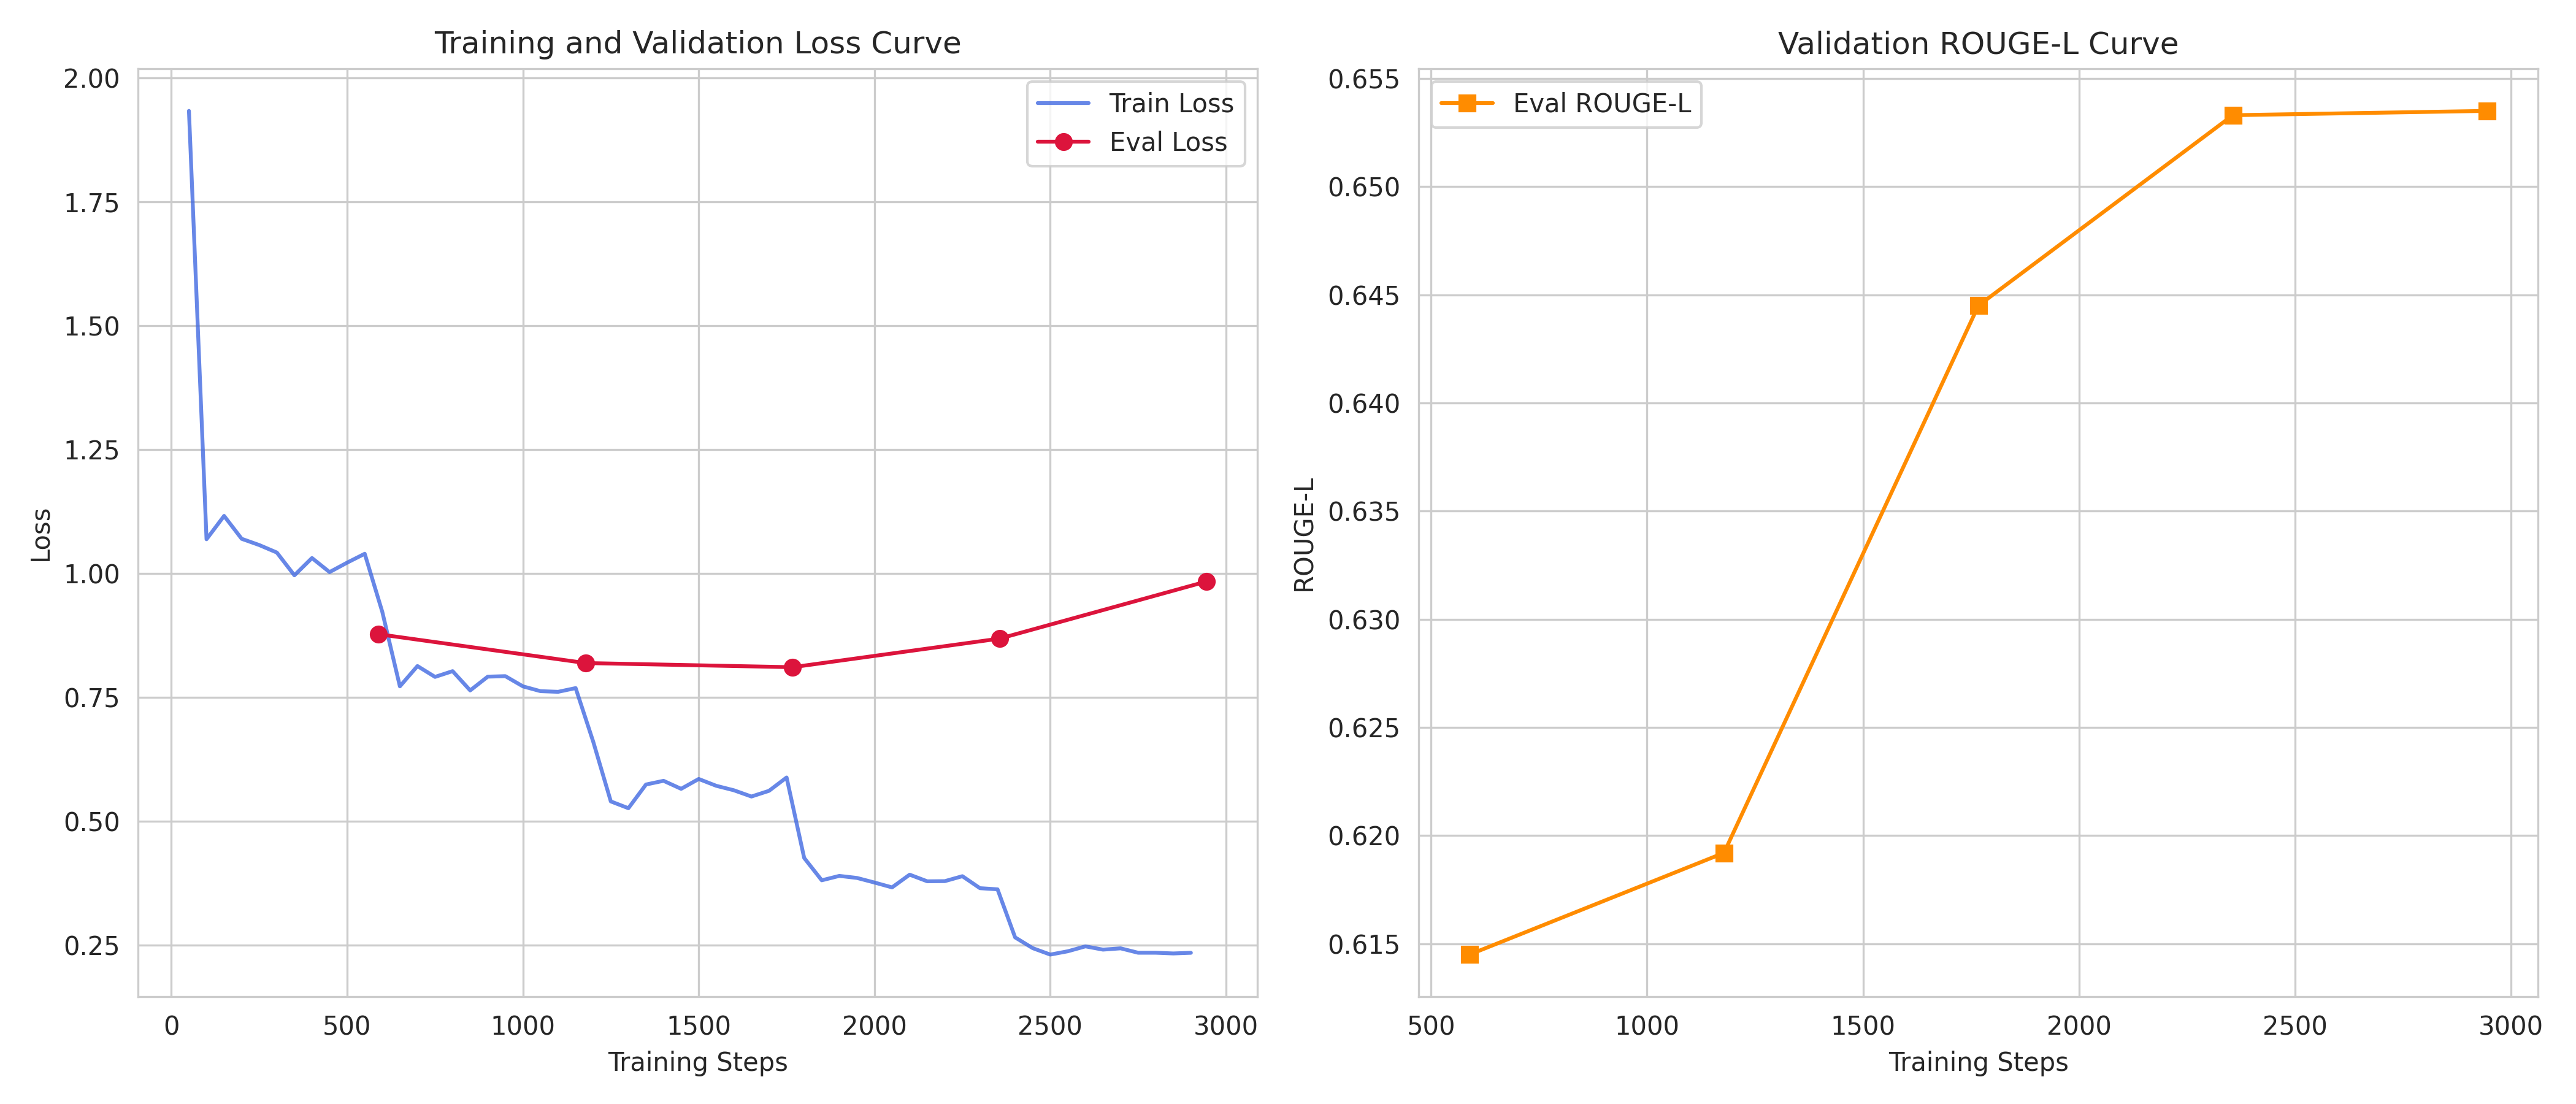
\includegraphics[width=0.85\textwidth]{figures/learning_curve_vit5.png}

    \caption{Đường cong học tập (Training/Validation Loss và Validation ROUGE-L) của mô hình ViT5-base}

    \label{fig:learning_curve}

\end{figure}



Từ Hình~\ref{fig:learning_curve}, hàm mất mát huấn luyện (Train Loss) có xu hướng giảm mạnh từ mức xấp xỉ $1,95$ và hội tụ về khoảng $0,25$ tại bước huấn luyện $3000$. Tuy nhiên, đối với tập kiểm định, hàm mất mát (Eval Loss) chỉ giảm đến giá trị cực tiểu khoảng $0,81$ tại bước $1800$ (tương đương epoch 3). Sau điểm này, Eval Loss bắt đầu tăng dần và chạm mức xấp xỉ $0,99$ ở bước $3000$, cho thấy mô hình đã bắt đầu xuất hiện hiện tượng quá khớp (overfitting) nhẹ. 
Song song đó, biểu đồ Validation ROUGE-L cho thấy hiệu suất chắp nối ngữ nghĩa bắt đầu từ $0,6145$, tăng trưởng mạnh mẽ và đạt trạng thái bão hòa (plateau) ở mức xấp xỉ $0,6536$ trong khoảng từ bước $2400$ đến bước $3000$. Sự bão hòa của chỉ số ROUGE-L kết hợp với đà tăng của Eval Loss ở giai đoạn cuối minh chứng rằng việc tiếp tục huấn luyện vượt quá bước $2400$ không mang lại giá trị gia tăng về chất lượng sinh văn bản, đồng thời việc hệ thống tự động thiết lập lưu \texttt{best\_model} dựa trên điểm ROUGE-L cao nhất thay vì Eval Loss thấp nhất là cần thiết để tối ưu hóa hiệu năng Abstractive QA.


\section{Nghiên cứu Ablation Study về chiến lược giải mã}
Chiến lược giải mã (decoding strategy) tại cấu phần generator có ảnh hưởng sống còn đến chất lượng văn bản y học sinh ra. Chúng tôi tiến hành nghiên cứu ablation study trên tập kiểm định (\texttt{val.json}) gồm $295$ mẫu để so sánh định lượng giữa hai phương pháp: giải mã tham lam (Greedy Decoding, $B=1$) và tìm kiếm chùm (Beam Search, $B=4$). Kết quả thực nghiệm được tổng hợp tại Bảng~\ref{tab:ablation_decoding}.

\begin{table}[H]
\centering
\caption{Kết quả Ablation Study về chiến lược giải mã trên tập kiểm định}
\label{tab:ablation_decoding}
\begin{tabular}{lccc}
\toprule
\textbf{Chiến lược giải mã} & \textbf{ROUGE-1} & \textbf{ROUGE-2} & \textbf{ROUGE-L} \\
\midrule
Greedy Decoding (beams=1) & 0,7188 & 0,5998 & 0,6527 \\
Beam Search (beams=4) & \textbf{0,7242} & \textbf{0,6069} & \textbf{0,6587} \\
\bottomrule
\end{tabular}
\end{table}

Kết quả tại Bảng~\ref{tab:ablation_decoding} chỉ ra rằng \textbf{Beam Search ($B=4$)} mang lại sự cải thiện đồng bộ trên tất cả các độ đo, cụ thể tăng khoảng \textbf{0,6\%} điểm ROUGE-L so với Greedy Decoding. Sự cải thiện này đạt được nhờ khả năng lưu giữ và đánh giá đồng thời nhiều giả thuyết dịch chuỗi tối ưu trên diện rộng, giúp mô hình tránh rơi vào các từ tối ưu cục bộ vốn dễ làm câu sinh ra bị cụt hoặc lặp từ. Tuy nhiên, Beam Search đòi hỏi chi phí tính toán và bộ nhớ lớn hơn. Trong các ứng dụng thực tế yêu cầu phản hồi tức thời với tài nguyên hạn chế, Greedy Decoding vẫn là một giải pháp thay thế rất khả thi nhờ tốc độ vượt trội mà không bị sụt giảm quá sâu về chất lượng.

\section{Phân tích định tính các trường hợp lỗi tiêu biểu (Failure Modes)}
Để hiểu rõ giới hạn nội tại và các điểm yếu y học của mô hình sinh, chúng tôi tiến hành phân tích định tính thủ công trên các mẫu dự đoán có điểm số thấp nhất từ tệp \texttt{worst\_10\_cases.csv}. Ba Failure Modes tiêu biểu đã được phát hiện và phân tích sâu sắc dưới góc độ y học lâm sàng:

\subsection{Lỗi lặp từ vô hạn (Repetitive Loop)}
\begin{tcolorbox}[colback=codebg, colframe=myblue, title={Ví dụ thực tế về lỗi lặp từ vô hạn do suy giảm tự hồi quy}]
\small\raggedright
\textbf{Câu hỏi:} Ngoài chấn thương đầu, còn có những nguyên nhân nào gây ra chóng mặt không?\par
\textbf{Tham chiếu:} Có rất nhiều nguyên nhân gây ra chóng mặt, như: rối loạn tiền đình, nhiễm trùng tai, tụt huyết áp, thiếu máu, sử dụng một số loại thuốc, v.v.\par
\textbf{Mô hình:} Có, chóng mặt có thể do chấn thương đầu, chấn thương đầu, chấn thương đầu, chấn thương đầu, chấn thương đầu, chấn thương đầu, chấn thương đầu, chấn thương đầu, chấn thương đầu, chấn thương đầu...
\end{tcolorbox}
\textbf{Biện luận y học và kỹ thuật:} Hiện tượng này xảy ra do sự suy giảm tự hồi quy (autoregressive degradation) của mô hình Seq2Seq khi sinh chuỗi dài. Khi phân phối xác suất của từ tiếp theo bị thống trị tuyệt đối bởi cụm từ vừa sinh ra trước đó (\textit{``chấn thương đầu''}), mô hình rơi vào trạng thái lặp vô hạn. Lỗi này cực kỳ nguy hiểm trong y tế vì nó triệt tiêu hoàn toàn thông tin hữu ích và gây trải nghiệm tồi tệ cho người dùng. Giải pháp khắc phục hiệu quả là thiết lập tham số hình phạt lặp từ khóa (\texttt{no\_repeat\_ngram\_size = 3}) hoặc áp dụng cơ chế giải mã đa dạng hóa (Contrastive Search) trong quá trình suy luận.

\subsection{Lỗi ảo tưởng thông tin lạc đề (Factual Hallucination \& Distraction)}
\begin{tcolorbox}[colback=codebg, colframe=myblue, title={Ví dụ thực tế về lỗi sinh thông tin ảo tưởng lạc đề}]
\small\raggedright
\textbf{Câu hỏi:} Nữ trinh tử và xấu hổ có đặc điểm gì giống nhau?\par
\textbf{Tham chiếu:} Cả hai đều thuộc họ Trinh nữ (Mimosaceae).\par
\textbf{Mô hình:} Cây xấu hổ có quả hình trứng hoặc hình bầu dục, có quả hơi cong, dài 7mm 10mm, đường kính khoảng 3mm, vỏ ngoài màu đen xám, có vằn nhăn, hai đầu tròn tày, một đầu có vết của cuống quả.
\end{tcolorbox}
\textbf{Biện luận y học và kỹ thuật:} Trong ví dụ này, mô hình đã tự sinh ra một mô tả cực kỳ chi tiết về quả của cây xấu hổ (được lưu giữ trong bộ nhớ tham số hoặc trích xuất từ phần ngữ cảnh dài liên quan đến cây xấu hổ). Tuy nhiên, mô hình hoàn toàn bỏ qua việc trả lời trọng tâm câu hỏi là chỉ ra \textit{điểm giống nhau} của hai loài thực vật y học (cùng thuộc họ Trinh nữ). Đây là lỗi mất tập trung ngữ cảnh (contextual distraction). Khi đối mặt với ngữ cảnh chứa quá nhiều chi tiết sinh học phức tạp, cơ chế Attention của mô hình bị quá tải và chọn lọc sai thông tin quan trọng. Điều này đòi hỏi retriever phải cắt gọt ngữ cảnh gọn gàng hơn trước khi đưa vào generator.

\subsection{Lỗi chi tiết quá mức gây sụt giảm độ đo (Overly Detailed Mismatch)}
\begin{tcolorbox}[colback=codebg, colframe=myblue, title={Ví dụ thực tế về câu trả lời y học chính xác bị chấm điểm thấp}]
\small\raggedright
\textbf{Câu hỏi:} Những bệnh lý nào tại tuyến yên có thể gây ra suy giảm tuyến thượng thận thứ phát?\par
\textbf{Tham chiếu:} U tuyến yên.\par
\textbf{Mô hình:} Những bệnh lý tại tuyến yên có thể gây ra suy giảm tuyến thượng thận thứ phát bao gồm: U tuyến yên hoặc vùng dưới đồi (một vùng ở não bộ), nhiễm trùng, ung thư, nhồi máu não, chấn thương sọ não, bất thường tuyến yên do đột biến gen.
\end{tcolorbox}
\textbf{Biện luận y học và kỹ thuật:} Đây là một trường hợp lỗi vô cùng đặc biệt. Về mặt y khoa học thuật, câu trả lời sinh ra bởi mô hình cực kỳ chính xác, đầy đủ và mang giá trị lâm sàng cao hơn rất nhiều so với câu trả lời tham chiếu quá ngắn gọn (\textit{``U tuyến yên''}). Tuy nhiên, do các độ đo ROUGE và BLEU chỉ tính toán dựa trên mức độ trùng khớp bề mặt n-gram của câu tham chiếu, mô hình bị chấm điểm ROUGE-L rất thấp (\textbf{0,1149}) và bị coi là lỗi \textit{Length Mismatch} (dài hơn $200\%$). Điều này vạch trần điểm hạn chế cốt lõi của các độ đo tự động truyền thống trong miền y tế - chúng thường phạt nặng những câu trả lời chi tiết và đầy đủ. Phát hiện này củng cố tầm quan trọng của việc sử dụng độ đo ngữ nghĩa BERTScore (đạt điểm rất cao trong trường hợp này) và kiểm chứng lâm sàng thủ công từ chuyên gia y tế.

\section{Công bố trọng số mô hình và mã nguồn mở}
Nhằm thúc đẩy khả năng tái lập nghiên cứu và đóng góp vào cộng đồng xử lý ngôn ngữ tự nhiên tiếng Việt, chúng tôi đã đóng gói toàn bộ trọng số mô hình tốt nhất (best checkpoint) của ViT5-base và đẩy lên hệ sinh thái HuggingFace Hub:
\begin{itemize}
    \item \textbf{Địa chỉ trọng số mô hình (HuggingFace Hub):} \href{https://huggingface.co/kimquoc/vit5-vimedaqa-medical-qa}{kimquoc/vit5-vimedaqa-medical-qa} hoặc \href{https://huggingface.co/ntthanh0307/vit5-vimedaq-medical-qa}{ntthanh0307/vit5-vimedaq-medical-qa}.
\end{itemize}
Trang model card đi kèm mô tả chi tiết thông số kiến trúc, bộ dữ liệu huấn luyện ViMedAQA, các chỉ số đánh giá thực nghiệm và đặc biệt là các điều khoản tuyên bố miễn trừ trách nhiệm pháp lý y khoa (medical disclaimer) bắt buộc khi ứng dụng mô hình vào thực tiễn.

\section{Triển khai ứng dụng Web Demo Gradio RAG}
Để trực quan hóa sức mạnh của mô hình trong thực tế, chúng tôi thiết kế và triển khai một ứng dụng web tương tác hoàn chỉnh dựa trên thư viện Gradio. Hệ thống được tích hợp kiến trúc Dense RAG tích hợp đầy đủ hai cấu phần Retriever (Bi-Encoder + FAISS) và Generator (ViT5-base) như đã mô tả ở Chương 3. Ảnh chụp màn hình giao diện thực tế của ứng dụng khi đang xử lý một truy vấn RAG y tế thành công được thể hiện tại Hình~\ref{fig:gradio_ui}.

\begin{figure}[H]
    \centering
    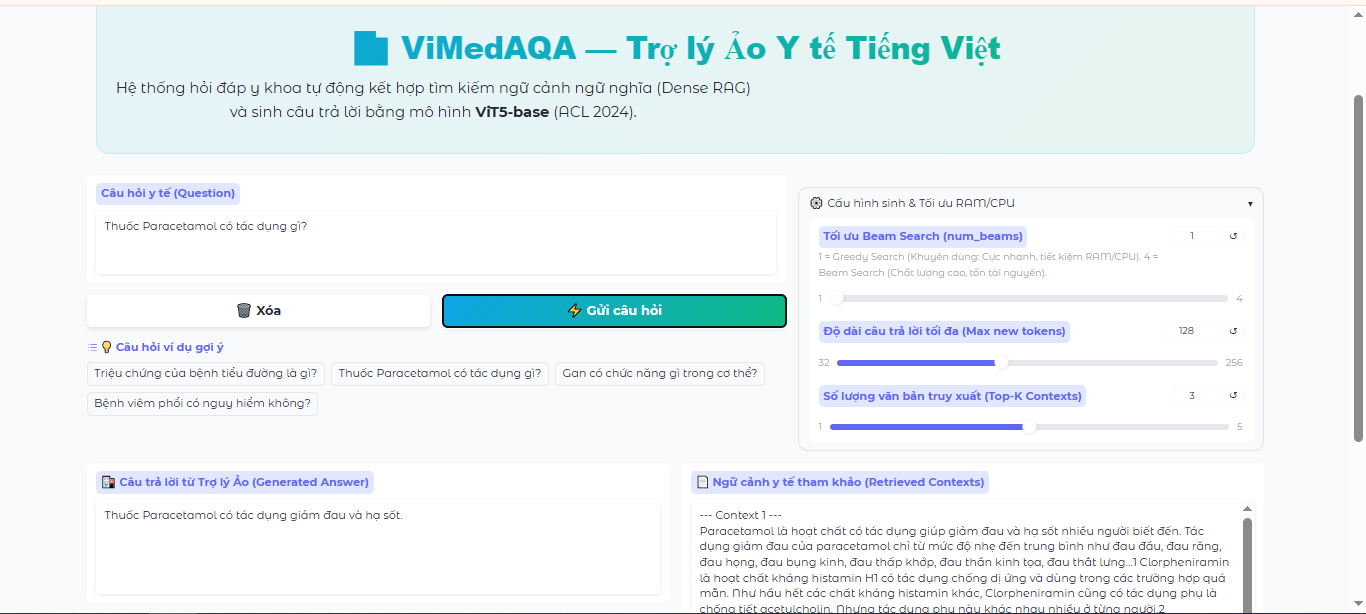
\includegraphics[width=0.85\textwidth]{figures/gradio_ui.png}
    \caption{Giao diện ứng dụng trợ lý ảo y tế ViMedAQA chạy thực tế trên HuggingFace Spaces}
    \label{fig:gradio_ui}
\end{figure}

Giao diện được tùy biến thiết kế (Custom CSS) với gam màu chủ đạo xanh ngọc và lục bảo (\texttt{linear-gradient(135deg, \#0ea5e9, \#10b981)}) mang lại cảm giác chuyên nghiệp, premium và tin cậy cho miền y tế. Người dùng có thể nhập câu hỏi tự nhiên ở khung bên trái, tinh chỉnh các thanh trượt cấu hình sinh (như số lượng chùm Beam Search $num\_beams$, số lượng ngữ cảnh truy xuất $top\_k$, và độ dài tối đa $max\_new\_tokens$). Khung bên phải sẽ hiển thị đồng thời hai kết quả trực quan: câu trả lời mạch lạc được sinh ra từ mô hình ViT5 và danh sách các văn bản ngữ cảnh y khoa tham khảo tương ứng được truy xuất từ FAISS để người dùng đối chiếu độ chính xác.

Ứng dụng demo được triển khai trực tuyến trên máy chủ đám mây của HuggingFace Spaces, phục vụ cộng đồng trải nghiệm thực tế tại địa chỉ:
\begin{itemize}
    \item \textbf{Liên kết ứng dụng Web Demo (HuggingFace Spaces):} \href{https://huggingface.co/spaces/kimquoc/vimedaqa-medical-qa}{kimquoc/vimedaqa-medical-qa}.
\end{itemize}